\documentclass[aps,pra,10pt,amsmath,notitlepage,letterpaper]{revtex4-1}
\usepackage{lmodern}
\usepackage{graphicx}
\usepackage{titletoc}
% \usepackage{showkeys}

\usepackage[bookmarksdepth=2,colorlinks=true,linkcolor=blue,
            citecolor=red,filecolor=magenta,urlcolor=blue,
            breaklinks=true]{hyperref}
\hypersetup{% PDF display options
   pdftitle={The Surface Second-Harmonic Generation Yield},
   pdfauthor={Sean M. Anderson},
   pdfsubject={Theory of SSHG in crystalline semiconductors.},
   pdfkeywords={nonlinear} {optics} {shg} {radiation} {semiconductors}
   {theoretical} {spectroscopy} {surface} {experiment}}

\begin{abstract}
In this manuscript, we will walk through the considerations for developing the
three layer (3-layer) model for the SSHG yield, which considers that the SH
conversion takes place in a thin layer just below the surface that lies under
the vacuum region and above the bulk of the material. We will then derive
explicit expressions for each of the four polarization configurations for the
incoming and outgoing fields. These expressions will be simplified by taking
into account the symmetry relations for the (111), (110), and (001) surfaces.
The reader can also consult the included Appendix that contains a wealth of
supplementary derivations for all the work contained in this manuscript.
\end{abstract}


\begin{document}

\title{The Surface Second-Harmonic Generation Yield}
    \author{Sean M. Anderson}
    \email{sma@cio.mx}
    \affiliation{Centro de Investigaciones en \'Optica, A.C.,
                 Le\'on 37150, Mexico}

    % \author{Yujin Cho}
    % \email{ycho@physics.utexas.edu}
    % \affiliation{Department of Physics,
    %              University of Texas at Austin,
    %              Austin, Texas 78712, USA}

    \author{Bernardo S. Mendoza}
    \email{bms@cio.mx}
    \affiliation{Centro de Investigaciones en \'Optica, A.C.,
                 Le\'on 37150, Mexico}

\maketitle
\tableofcontents


%%%%%%%%%%%%%%%%%%%%%%%%%%%%%%%%%%%%%%%%%%%%%%%%%%%%%%%%%%%%%%%%%%%%%%%%%%%%%%%%
%%%%%%%%%%%%%%%%%%%%%%%%%%%%%%%%%%%%%%%%%%%%%%%%%%%%%%%%%%%%%%%%%%%%%%%%%%%%%%%%

\section{The Three Layer Model for the SSHG Yield}\label{sec:3layersshg}

In this section, we will derive the formulas required for the calculation of the
SSHG yield, defined by
\begin{equation}\label{eq:rintensities}
\mathcal{R}(\omega)=\frac{I(2\omega)}{I^2(\omega)},
\end{equation}
with the intensity given by \cite{boyd, sutherland}
\begin{equation}\label{eq:intensity}
I(\omega)=
\left\{
\begin{array}{cc}
\frac{c}{2\pi}n(\omega)|E(\omega)|^{2} & \text{(CGS units)} \\\\
2\epsilon_{0}c\, n(\omega)|E(\omega)|^{2} & \text{(MKS units)}
\end{array}
\right.,
\end{equation}
where $n(\omega)=\sqrt{\epsilon(\omega)}$ is the index of refraction
($\epsilon(\omega)$ is the dielectric function), $\epsilon_{0}$ is the vacuum
permittivity, and $c$ the speed of light in vacuum.

There are several ways to calculate $\mathcal{R}(\omega)$, one of which is the
procedure followed by Cini \cite{ciniPRB91}. This approach calculates the
nonlinear susceptibility and at the same time the radiated fields. However, we
present an alternative derivation based on the work of Mizrahi and Sipe
\cite{mizrahiJOSA88}, since the derivation of the 3-layer model is
straightforward. In this scheme, the surface is represented by three regions or
layers. The first layer is the vacuum region (denoted by $v$) with a dielectric
function $\epsilon_{v}(\omega)=1$ from where the fundamental electric field
$\mathbf{E}_{v}(\omega)$ impinges on the material. The second layer is a thin
layer (denoted by $\ell$) of thickness $d$ characterized by a dielectric
function $\epsilon_{\ell}(\omega)$. It is in this layer where the SHG takes
place. The third layer is the bulk region denoted by $b$ and characterized by
$\epsilon_{b}(\omega)$. Both the vacuum and bulk layers are semi-infinite (see
Fig. \ref{fig:MR3layer2w}).

\begin{figure}[b]
\centering 
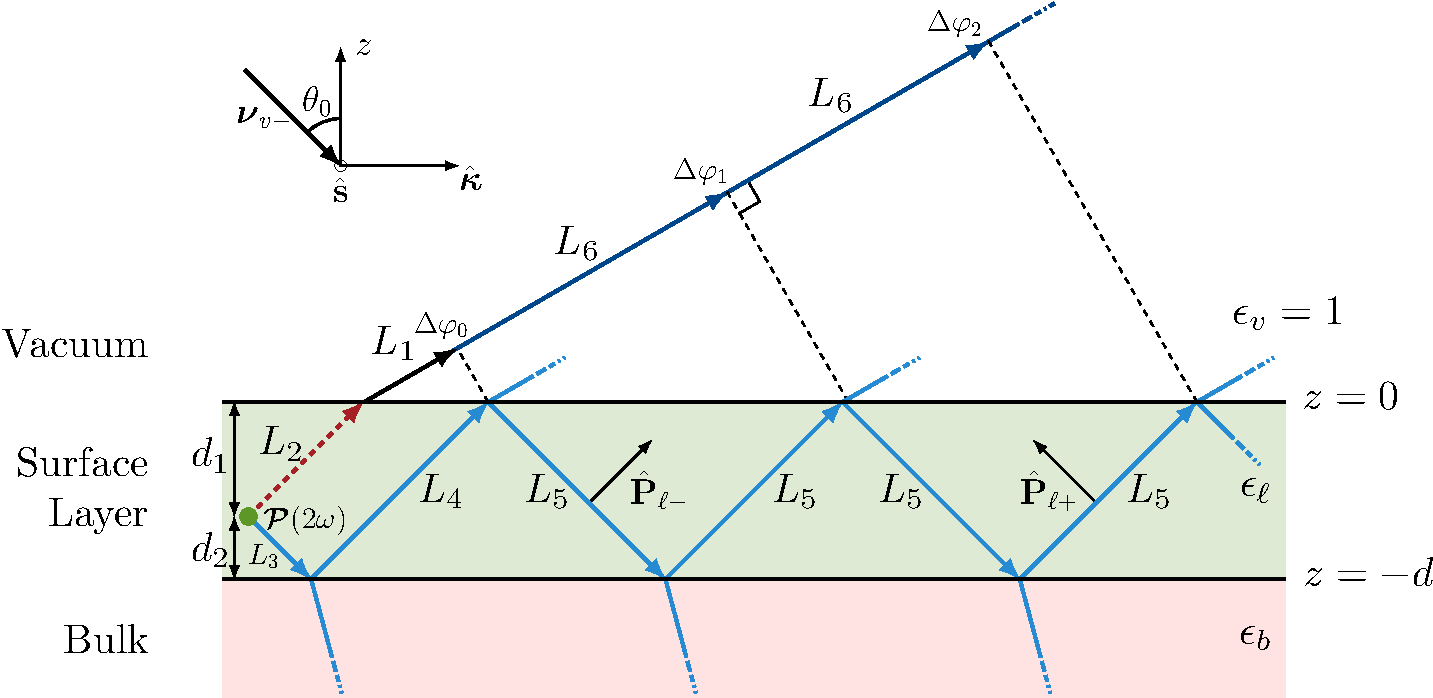
\includegraphics[width=0.65\linewidth]{../../content/figures/diag-3layer_MR_2w}
\caption[Sketch of the three layer model for SHG.]
{Sketch of the three layer model for SHG. The vacuum region ($v$) is on top with
$\epsilon_{v}=1$; the layer $\ell$ of thickness $d = d_{1} + d_{2}$, is
characterized by $\epsilon_{\ell}(\omega)$, and it is where the SH polarization
sheet $\boldsymbol{\mathcal{P}}_{\ell}(2\omega)$ is located at $z_{\ell} =
d_{1}$. The bulk $b$ is described by $\epsilon_{b}(\omega)$. The arrows point
along the direction of propagation, and the $p$-polarization unit vector,
$\hat{\mathbf{P}}_{\ell -(+)}$, along the downward (upward) direction is denoted
with a thick arrow. The $s$-polarization unit vector $\hat{\mathbf{s}}$, points
out of the page. The fundamental field $\mathbf{E}_{v}(\omega)$ is incident from
the vacuum side along the $\hat{\boldsymbol{\kappa}}z$-plane, with $\theta_{0}$
its angle of incidence and $\boldsymbol{\nu}_{v-}$ its wave vector.
$\Delta\varphi_{i}$ denotes the phase difference between the multiple reflected
beams and the first layer-vacuum transmitted beam, denoted by the dashed-red
arrow (of length $L_{2}$) followed by the solid black arrow (of length $L_{1}$).
The dotted lines in the vacuum region are perpendicular to the beam extended
from the solid black arrow (denoted by solid blue arrows of length $L_{6}$).}
\label{fig:MR3layer2w}
\end{figure}

To model the electromagnetic response of the 3-layer model, we follow Ref.
\cite{mizrahiJOSA88} and assume a polarization sheet located at $z_{\beta}$, of
the form
\begin{equation}\label{eq:psheet}
\mathbf{P}(\mathbf{r},t) = \boldsymbol{\mathcal{P}}
e^{i\boldsymbol{\kappa}\cdot\mathbf{R}}e^{-i\omega t}\delta(z - z_{\beta}) 
+ \mathrm{c.c.},
\end{equation}
where $\mathbf{R}=(x,y)$, $\boldsymbol{\kappa}$ is the component of the wave
vector $\boldsymbol{\nu}^{\phantom{a}}_{\beta}$ parallel to the surface, and
$z_{\beta}$ is the position of the sheet within medium $\beta$, and
$\boldsymbol{\mathcal{P}}$ is the position-independent polarization. Ref.
\cite{sipeJOSAB87} demonstrates that the solution of the Maxwell equations for
the radiated fields $E_{\beta,p\pm}$, and $E_{\beta,s}$ with
$\mathbf{P}(\mathbf{r},t)$ as a source at points $z\neq 0$, can be written as
\begin{equation}\label{eq:solmaxwell}
(E_{\beta,p\pm},E_{\beta,s}) = 
(\frac{\gamma i\tilde{\omega}^2}{\tilde{w}_{\beta}}
\,\hat{\mathbf{p}}_{\beta\pm}\cdot\boldsymbol{\mathcal{P}},
\frac{\gamma i\tilde{\omega}^2}{\tilde{w}_{\beta}}
\,\hat{\mathbf{s}}\cdot\boldsymbol{\mathcal{P}}),
\end{equation} 
where $\gamma=2\pi$ in CGS units or $\gamma=1/2\epsilon_{0}$ in MKS units, and
$\tilde{\omega}=\omega/c$. Also, $\hat{\mathbf{s}}$ and
$\hat{\mathbf{p}}_{\beta\pm}$ are the unit vectors for the $s$ and $p$
polarizations of the radiated field, respectively. The $\pm$ refers to upward
($+$) or downward ($-$) direction of propagation within medium $\beta$, as shown
in Fig. \ref{fig:MR3layer2w}. Also,
$\tilde{w}^{\phantom{a}}_{\beta}(\omega)=\tilde{\omega}w^{\phantom{a}}_{\beta}$,
where
\begin{equation}\label{eq:r4}
\hat{\mathbf{p}}^{\phantom{A}}_{\beta\pm}(\omega) =
  \frac{\kappa(\omega)\hat{\mathbf{z}}\mp 
  \tilde{w}^{\phantom{A}}_{\beta}(\omega)\hat{\boldsymbol{\kappa}}} 
  {\tilde{\omega} n^{\phantom{A}}_{\beta}(\omega)}
= \frac{\sin\theta_{0}\hat{\mathbf{z}}\mp 
  w^{\phantom{A}}_{\beta}(\omega)\hat{\boldsymbol{\kappa}}} 
  {n^{\phantom{A}}_{\beta}(\omega)},
\end{equation}
with
\begin{equation}\label{eq:wavevector}
w^{\phantom{a}}_{\beta}(\omega) = 
\big(\epsilon^{\phantom{a}}_{\beta}(\omega) - \sin^{2}\theta_{0}\big)^{1/2},
\end{equation}
$\theta_{0}$ is the angle of incidence of $\mathbf{E}_{v}(\omega)$,
$\kappa(\omega)=\vert\boldsymbol{\kappa}\vert = \tilde{\omega}\sin\theta_{0}$,
$n^{\phantom{A}}_{\beta}(\omega)=\sqrt{\epsilon^{\phantom{A}}_{\beta}(\omega)}$
is the index of refraction of medium $\beta$, and $z$ is the direction
perpendicular to the surface that points towards the vacuum. If we consider the
plane of incidence along the $\boldsymbol{\kappa}z$ plane, then
\begin{equation}\label{eq:mc1}
\hat{\boldsymbol{\kappa}} = \cos\phi\hat{\mathbf{x}} + \sin\phi\hat{\mathbf{y}},
\end{equation}
and
\begin{equation}\label{eq:mmc2}
\hat{\mathbf{s}} = -\sin\phi\hat{\mathbf{x}} + \cos\phi\hat{\mathbf{y}},
\end{equation}
where $\phi$ is the azimuthal angle with respect to the $x$ axis.

In the 3-layer model the nonlinear polarization responsible for the SHG is
immersed in the thin layer ($\beta=\ell$), and is given by
\begin{equation}\label{eq:tres}
\mathcal{P}^{\mathrm{a}}_{\ell}(2\omega) =
\left\{
\begin{array}{cc}
\chi^{\mathrm{abc}}_{\mathrm{surface}}(-2\omega;\omega,\omega)
    E^{\mathrm{b}}(\omega)E^{\mathrm{c}}(\omega)
    & \text{(CGS units)}\\\\
\epsilon_{0}\chi^{\mathrm{abc}}_{\mathrm{surface}}(-2\omega;\omega,\omega)
    E^{\mathrm{b}}(\omega)E^{\mathrm{c}}(\omega)
    & \text{(MKS units)}
\end{array}
\right.,
\end{equation}
where $\boldsymbol{\chi}_{\mathrm{surface}}(-2\omega;\omega,\omega)$ is the
dipolar surface nonlinear susceptibility tensor that we have derived in detail
in Refs. \cite{andersonPRB15, andersonthesis}, and the Cartesian indices
$\mathrm{a,b,c}$ are summed over if repeated. As we mentioned before,
$\chi^{\mathrm{abc}}(-2\omega;\omega,\omega) =
\chi^{\mathrm{acb}}(-2\omega;\omega,\omega)$ is the intrinsic permutation
symmetry due to the fact that SHG is degenerate in $E^{\mathrm{b}}(\omega)$ and
$E^{\mathrm{c}}(\omega)$. As in Ref. \cite{mizrahiJOSA88}, we consider the
polarization sheet (Eq. \eqref{eq:psheet}) to be oscillating at some frequency
$\omega$ in order to properly express Eqs.
\eqref{eq:solmaxwell}-\eqref{eq:mmc2}. However, in the following we find it
convenient to use $\omega$ exclusively to denote the fundamental frequency and
$\boldsymbol{\kappa}$ to denote the component of the incident wave vector
parallel to the surface. The generated nonlinear polarization is oscillating at
$\Omega = 2\omega$ and will be characterized by a wave vector parallel to the
surface $\mathbf{K} = 2\boldsymbol{\kappa}$. We can carry over Eqs.
\eqref{eq:psheet}-\eqref{eq:mmc2} simply by replacing the lowercase symbols
($\omega,\tilde{\omega},\boldsymbol{\kappa},n^{\phantom{A}}_{\beta},
\tilde{w}^{\phantom{A}}_{\beta},w^{\phantom{A}}_{\beta},
\hat{\mathbf{p}}^{\phantom{A}}_{\beta\pm},\hat{\mathbf{s}}$) with uppercase
symbols ($\Omega,\tilde{\Omega},\mathbf{K},N^{\phantom{A}}_{\beta},
\tilde{W}^{\phantom{A}}_{\beta},W^{\phantom{A}}_{\beta},
\hat{\mathbf{P}}_{\beta\pm},\hat{\mathbf{S}}$), all evaluated at $2\omega$. Of
course, we always have that $\hat{\mathbf{S}}=\hat{\mathbf{s}}$.

From Fig. \ref{fig:MR3layer2w}, we observe the propagation of the SH field as it
is refracted at the layer-vacuum interface ($\ell v$), and  reflected multiple
times from the layer-bulk ($\ell b$) and layer-vacuum ($\ell v$) interfaces.
Thus, we can define
\begin{equation}\label{eq:r5}
\mathbf{T}^{\ell v}
= \hat{\mathbf{s}}T_{s}^{\ell v}\hat{\mathbf{s}} 
+ \hat{\mathbf{P}}_{v+}T_{p}^{\ell v} \hat{\mathbf{P}}_{\ell +},
\end{equation}
as the transmission tensor for the $\ell v$ interface,
\begin{equation}\label{eq:r6}
\mathbf{R}^{\ell b}
= \hat{\mathbf{s}}R_{s}^{\ell b}\hat{\mathbf{s}}
+ \hat{\mathbf{P}}_{\ell +}R_{p}^{\ell b} \hat{\mathbf{P}}_{\ell -},
\end{equation} 
as the reflection tensor for the $\ell b$ interface, and
\begin{equation}\label{eq:r6b}
\mathbf{R}^{\ell v}
= \hat{\mathbf{s}}R_{s}^{\ell v}\hat{\mathbf{s}}
+ \hat{\mathbf{P}}_{\ell -}R_{p}^{\ell v} \hat{\mathbf{P}}_{\ell +},
\end{equation} 
as the reflection tensor for the $\ell v$ interface. The Fresnel factors in
uppercase letters, $T^{ij}_{s,p}$ and $R^{ij}_{s,p}$, are evaluated at $2\omega$
from the following well known formulas \cite{jacksonbook}
\begin{equation}\label{eq:e.f1}
\begin{split}
t_{s}^{ij}(\omega) &=
\frac{2w_{i}(\omega)}{w_{i}(\omega) + w_{j}(\omega)},
\quad\quad  
t_{p}^{ij}(\omega) =
\frac{2w_{i}(\omega)\sqrt{\epsilon_{i}(\omega)\epsilon_j(\omega)}}
     {w_{i}(\omega)\epsilon_{j}(\omega) + w_{j}(\omega)\epsilon_{i}(\omega)},\\
r_{s}^{ij}(\omega) &=
\frac{w_{i}(\omega) - w_{j}(\omega)}
     {w_{i}(\omega) + w_{j}(\omega)},
\quad\quad 
r_{p}^{ij}(\omega) =
\frac{w_{i}(\omega)\epsilon_{j}(\omega) - w_{j}\epsilon_{i}(\omega)}
     {w_{i}(\omega)\epsilon_{j}(\omega) + w_{j}(\omega)\epsilon_{i}(\omega)}. 
\end{split}
\end{equation}
With these expressions we easily derive the following useful relations,
\begin{equation}\label{eq:mf}
\begin{split}
1 + r^{\ell b}_{s} &= t^{\ell b}_{s},\\
1 + r^{\ell b}_{p} &= \frac{n_{b}}{n_{\ell}}t^{\ell b}_{p},\\
1 - r^{\ell b}_{p} &= \frac{n_{\ell}}{n_{b}}\frac{w_{b}}{w_{\ell}}
                      t^{\ell b}_{p},\\
t^{\ell v}_{p} &= \frac{w_{\ell}}{w_{v}}t^{v\ell}_{p},\\
t^{\ell v}_{s} &= \frac{w_{\ell}}{w_{v}}t^{v\ell}_{s}.
\end{split}
\end{equation}


%%%%%%%%%%%%%%%%%%%%%%%%%%%%%%%%%%%%%%%%%%%%%%%%%%%%%%%%%%%%%%%%%%%%%%%%%%%%%%%%

\subsection{Multiple SHG Reflections}

The SH field $\mathbf{E}(2\omega)$ radiated by the SH polarization
$\boldsymbol{\mathcal{P}}_{\ell}(2\omega)$ will radiate directly into the vacuum
and the bulk, where it will be reflected back at the layer-bulk interface into
the thin layer. This beam will be transmitted and reflected multiple times, as
shown in Fig. \ref{fig:MR3layer2w}. As the two beams propagate, a phase
difference will develop between them according to
\begin{equation}\label{eq:m99}
\begin{split}
\Delta\varphi_{m} 
&= \tilde{\Omega}
\Big(
(L_{3} + L_{4} + 2mL_{5})N_{\ell}
 - \big(L_{2}N_{\ell} + (L_{1} + mL_{6})N_{v}\big)
\Big)\\
&= \delta_{0} + m\delta,\quad m=0,1,2,\ldots,
\end{split}
\end{equation}
where
\begin{equation}\label{eq:delta0}
\delta_{0} =
8\pi\left(\frac{d_{2}}{\lambda_{0}}\right)W_{\ell},
\end{equation}
and
\begin{equation}\label{eq:delta}
\delta = 8\pi
\left(\frac{d}{\lambda_{0}}\right)W_{\ell},
\end{equation}
where $\lambda_{0}$ is the wavelength of the fundamental field in the vacuum,
$W_{\ell}$ is described in Eq. \eqref{eq:wavevector}, $d$ is the
thickness of layer $\ell$, and $d_{2}$ is the distance between
$\boldsymbol{\mathcal{P}}_{\ell}(2\omega)$ and the $\ell b$ interface (see Fig.
\ref{fig:MR3layer2w}). We see that $\delta_{0}$ is the phase difference of the
first and second transmitted beams, and $m\delta$ that of the first and third
($m = 1$), first and fourth ($m = 2$), and so on. Note that the thickness $d$ of
the layer $\ell$ enters through the phase $\delta$, and the position $d_{2}$ of
the nonlinear polarization $\mathbf{P}(\mathbf{r},t)$ (Eq. \eqref{eq:psheet})
enters through $\delta_{0}$. In particular, $d_{2}$ could be used as a variable
to study the effects of multiple reflections on the SSHG yield
$\mathcal{R}(2\omega)$.

To take into account the multiple reflections of the generated SH field in the
layer $\ell$, we proceed as follows. I include the algebra for the $p$-polarized
SH field, and the $s$-polarized field could be worked out along the same steps.
The $p$-polarized $\mathbf{E}_{\ell,p}(2\omega)$ field reflected multiple times
is given by
\begin{equation}\label{eq:E2wcomplete}
\begin{split}
\mathbf{E}_{\ell,p}(2\omega) 
&= E_{\ell,p+}(2\omega)\mathbf{T}^{\ell v}\cdot\hat{\mathbf{P}}_{\ell +}
 + E_{\ell,p-}(2\omega)\mathbf{T}^{\ell v}
\cdot\mathbf{R}^{\ell b}\cdot\hat{\mathbf{P}}_{\ell-}e^{i\Delta\varphi_{0}}\\
&+ E_{\ell,p-}(2\omega)\mathbf{T}^{\ell v}
\cdot\mathbf{R}^{\ell b}\cdot\mathbf{R}^{\ell v}
\cdot\mathbf{R}^{\ell b}\cdot\hat{\mathbf{P}}_{\ell-}e^{i\Delta\varphi_{1}}
\\
&+ E_{\ell,p-}(2\omega)\mathbf{T}^{\ell v}
\cdot\mathbf{R}^{\ell b}\cdot\mathbf{R}^{\ell v}
\cdot\mathbf{R}^{\ell b}\cdot\mathbf{R}^{\ell v}
\cdot\mathbf{R}^{\ell b}\cdot\hat{\mathbf{P}}_{\ell-}e^{i\Delta\varphi_{2}}
+\cdots\\
&= E_{\ell,p+}(2\omega)\mathbf{T}^{\ell v}\cdot\hat{\mathbf{P}}_{\ell +}
+ E_{\ell,p-}(2\omega) \mathbf{T}^{\ell v}
\cdot\sum_{m=0}^\infty  
\big(
\mathbf{R}^{\ell b}\cdot\mathbf{R}^{\ell v} 
e^{i\delta}\Big)^m 
\cdot\mathbf{R}^{\ell b}\cdot\hat{\mathbf{P}}_{\ell-}e^{i\delta_{0}}.
\end{split}
\end{equation}
From Eqs. \eqref{eq:r5} - \eqref{eq:r6b} it is easy to show that
\begin{equation*}\label{eq:m1}
\mathbf{T}^{\ell v}\cdot
\Big(\mathbf{R}^{\ell b}\cdot\mathbf{R}^{\ell v}\Big)^{n}\cdot
\mathbf{R}^{\ell b}
= \hat{\mathbf{s}}T^{\ell v}_{s}
  \Big(R^{\ell b}_{s}R^{\ell v}_{s}\Big)^{n}R^{\ell b}_{s}\hat{\mathbf{s}}
+ \hat{\mathbf{P}}_{v+}T^{\ell v}_{p}\Big(R^{\ell b}_{p}R^{\ell v}_{p}\Big)^n 
  R^{\ell b}_{p} 
\hat{\mathbf{P}}_{\ell-},
\end{equation*}
then,
\begin{equation}\label{eq:E2wreduced}
\mathbf{E}_{\ell,p}(2\omega) 
= \hat{\mathbf{P}}_{\ell +}T^{\ell v}_{p}
\Big(
E_{\ell,p+}(2\omega) +
\frac{R^{\ell b}_{p}e^{i\delta_{0}}}{1 + R^{v\ell}_{p}R^{\ell b}_{p}e^{i\delta}}
E_{\ell,p-}(2\omega) 
\Big),
\end{equation}
where we used $R^{ij}_{s,p} = -R^{ji}_{s,p}$. Using Eq. \eqref{eq:solmaxwell}
and \eqref{eq:mf}, we can readily write
\begin{equation}\label{eq:mr8}
\mathbf{E}_{\ell,p}(2\omega) =
\frac{\gamma i\tilde{\Omega}}{W_{\ell}}\mathbf{H}_{\ell}\cdot
\boldsymbol{\mathcal{P}}_{\ell}(2\omega),
\end{equation}
where
\begin{equation}\label{eq:mr9}
\mathbf{H}_{\ell}
= \frac{W_\ell}{W_v}
\left[
\hat{\mathbf{s}}\,T_{s}^{v\ell}
\left(1+ R^{M}_{s}\right)\hat{\mathbf{s}} + \hat{\mathbf{P}}_{v+}T_{p}^{v\ell}
\left(\hat{\mathbf{P}}_{\ell +} + R^{M}_{p}\hat{\mathbf{P}}_{\ell -}\right)
\right],
\end{equation}
and
\begin{equation}\label{m61}
R^{M}_{\mathrm{i}}\equiv
\frac{R^{\ell b}_{\mathrm{i}}e^{i\delta_{0}}}
     {1+R^{v\ell}_{\mathrm{i}} R^{\ell b}_{\mathrm{i}}e^{i\delta}},
     \quad \mathrm{i}=s,p,
\end{equation}
is defined as the multiple ($M$) reflection coefficient. This coefficient
depends on the thickness $d$ of layer $\ell$, and most importantly on the
position $d_{2}$ of $\boldsymbol{\mathcal{P}}_{\ell}(2\omega)$ within this
layer. The final results will depend on both $d$ and $d_{2}$. However, using Eq.
\eqref{eq:delta0} we can also define an average $\bar{R}^{M}_{\mathrm{i}}$ as
\begin{equation}\label{eq:mcave}
\bar{R}^{M}_{\mathrm{i}}\equiv 
\frac{1}{d}\int_{0}^{d}
\frac{R^{\ell b}_{\mathrm{i}}e^{i(8\pi W_{\ell}/\lambda_{0})x}}
{1 + R^{v\ell}_{\mathrm{i}}R^{\ell b}_{\mathrm{i}}e^{i\delta}}\,dx
= \frac{R^{\ell b}_{\mathrm{i}}e^{i\delta/2}}
{1 + R^{v\ell}_{\mathrm{i}}R^{\ell b}_{\mathrm{i}}e^{i\delta}}
\,\mathrm{sinc}(\delta/2),
\end{equation}
that only depends on $d$ through the $\delta$ term from Eq. \eqref{eq:delta}.

To connect with the work in Ref. \cite{mizrahiJOSA88}, where
$\boldsymbol{\mathcal{P}}(2\omega)$ is located on top of the vacuum-surface
interface and only the vacuum radiated beam and the first (and only) reflected
beam need be considered, we take $\ell = v$ and $d_{2} = 0$, then $T^{\ell v} =
1$, $R^{v\ell} = 0$ and $\delta_{0} = 0$, with which $R^{M}_{\mathrm{i}} =
R^{vb}_{\mathrm{i}}$. Thus, Eq. \eqref{eq:mr9} coincides with Eq. (3.8) of Ref.
\cite{mizrahiJOSA88}.


%%%%%%%%%%%%%%%%%%%%%%%%%%%%%%%%%%%%%%%%%%%%%%%%%%%%%%%%%%%%%%%%%%%%%%%%%%%%%%%%

\subsection{Multiple Reflections for the Linear Field}

For a more complete formulation, we must also consider the multiple reflections
of the fundamental field $\mathbf{E}_{\ell}(\omega)$ inside the thin $\ell$
layer. In Fig. \ref{fig:MR3layer1w} we present the situation where
$\mathbf{E}_{v}(\omega)$ impinges from the vacuum side with an angle of
incidence $\theta_{0}$. As the first transmitted beam is multiply reflected from
the $\ell b$ and the $\ell v$ interfaces, it accumulates a phase difference of
$n\varphi$ (with $n=1,2,3,\ldots$), and $\varphi$ is given by
\begin{equation}\label{mphi}
\begin{split}
\varphi &= \frac{\omega}{c}(2L_{1}n_{\ell} - L_{2}n_{v})\\
&= 4\pi\left(\frac{d}{\lambda_{0}}\right)w_{\ell},
\end{split}
\end{equation}
where $n_{v}=1$. We need Eqs. \eqref{eq:r6} and \eqref{eq:r6b} for $1\omega$, and
also need
\begin{equation}\label{eq:mvv}
\mathbf{t}^{v\ell}
= \hat{\mathbf{s}}t_{s}^{v\ell}\hat{\mathbf{s}} 
+ \hat{\mathbf{p}}_{\ell -}t_{p}^{v\ell}\hat{\mathbf{p}}_{v-},
\end{equation}
to write
\begin{align}\label{eq:mcvew}
\mathbf{E}_{\ell}(\omega)
&= E_{0}
\Big[
\mathbf{t}^{v\ell} + \mathbf{r}^{\ell b}\cdot\mathbf{t}^{v\ell}e^{i\varphi}
 + \mathbf{r}^{\ell b}\cdot\mathbf{r}^{\ell v}\cdot
   \mathbf{r}^{\ell b}\cdot\mathbf{t}^{v\ell} e^{i2\varphi}
 + \mathbf{r}^{\ell b}\cdot\mathbf{r}^{\ell v}\cdot
   \mathbf{r}^{\ell b}\cdot\mathbf{r}^{\ell v}\cdot
   \mathbf{r}^{\ell b}\cdot\mathbf{t}^{v\ell} e^{i3\varphi}
 + \cdots
\Big]\cdot\hat{\mathbf{e}}^{\mathrm{i}}\nonumber\\
&= E_{0}
\Big[
1 + \Big(1 + \mathbf{r}^{\ell b}\cdot\mathbf{r}^{\ell v}e^{i\varphi}
+ (\mathbf{r}^{\ell b}\cdot\mathbf{r}^{\ell v})^2e^{i2\varphi}+\cdots\Big)\cdot
\mathbf{r}^{\ell b}e^{i\varphi}
\Big]
\cdot\mathbf{t}^{v\ell}\cdot\hat{\mathbf{e}}^{\mathrm{i}}\nonumber\\
&= E_{0}
\Big[
\hat{\mathbf{s}} t^{v\ell}_{s}(1+r^{M}_{s})\hat{\mathbf{s}} 
+ t^{v\ell}_{p}
\left(\hat{\mathbf{p}}_{\ell-}+\hat{\mathbf{p}}_{\ell+}r^{M}_{p}\right)
\hat{\mathbf{p}}_{v-}
\Big]\cdot\hat{\mathbf{e}}^{\mathrm{i}},
\end{align}
where $E_{0}$ is the intensity of the fundamental field, and
$\hat{\mathbf{e}}^{\mathrm{i}}$ is the unit vector of the incoming polarization,
with $\mathrm{i} = s,p$, and then, $\hat{\mathbf{e}}^{s}=\hat{\mathbf{s}}$ and
$\hat{\mathbf{e}}^{p}=\hat{\mathbf{p}}_{v-}$. Also,
\begin{equation}\label{mvrm}
r^{M}_{\mathrm{i}} \equiv
\frac{r^{\ell b}_{\mathrm{i}}e^{i\varphi}}{1+r^{v\ell}_{\mathrm{i}}
r^{\ell b}_{\mathrm{i}}e^{i\varphi}}, \quad \mathrm{i}=s,p.
\end{equation}
$r^{M}_{\mathrm{i}}$ is defined as the multiple (M) reflection coefficient for
the fundamental field. We define $\mathbf{E}^{\mathrm{i}}_{\ell}(\omega)\equiv
E_{0}\mathbf{e}^{\omega,\mathrm{i}}_{\ell}$ ($\mathrm{i}=s,p$), where
\begin{equation}\label{eq:mcvew2}
\mathbf{e}^{\omega,\mathrm{i}}_\ell 
= \Big[\hat{\mathbf{s}} t^{v\ell}_s(1+r^M_s)\hat{\mathbf{s}} 
+ t^{v\ell}_p\left(\hat{\mathbf{p}}_{\ell-}+\hat{\mathbf{p}}_{\ell+}r^{M}_p 
\right)\hat{\mathbf{p}}_{v-}
\Big]\cdot\hat{\mathbf{e}}^{\mathrm{i}},
\end{equation}
and using Eqs. \eqref{eq:r4}, \eqref{eq:mc1}, and \eqref{eq:mmc2} we obtain that
\begin{equation}\label{eq:vec1wcomplete}
\mathbf{e}^{\omega,i}_{\ell}
=
\Bigg[
t^{v\ell}_{s} r^{M+}_{s}
\left(- \sin\phi\hat{\mathbf{x}} + \cos\phi\hat{\mathbf{y}}\right)
\hat{\mathbf{s}}
+
\frac{t^{v\ell}_{p}}{n_{\ell}}
\left( 
  r^{M+}_{p}\sin\theta_{0}\hat{\mathbf{z}}
+ r^{M-}_{p}w_{\ell}\cos\phi\hat{\mathbf{x}}
+ r^{M-}_{p}w_{\ell}\sin\phi\hat{\mathbf{y}}
\right)
\hat{\mathbf{p}}_{v-}
\Bigg]
\cdot \hat{\mathbf{e}}^{\mathrm{i}},
\end{equation} 
where
\begin{equation}\label{eq:mvc}
r^{M\pm}_{\mathrm{i}}=1\pm r^{M}_{\mathrm{i}},\quad \mathrm{i} = s,p.
\end{equation}

\begin{figure}[t]
\centering 
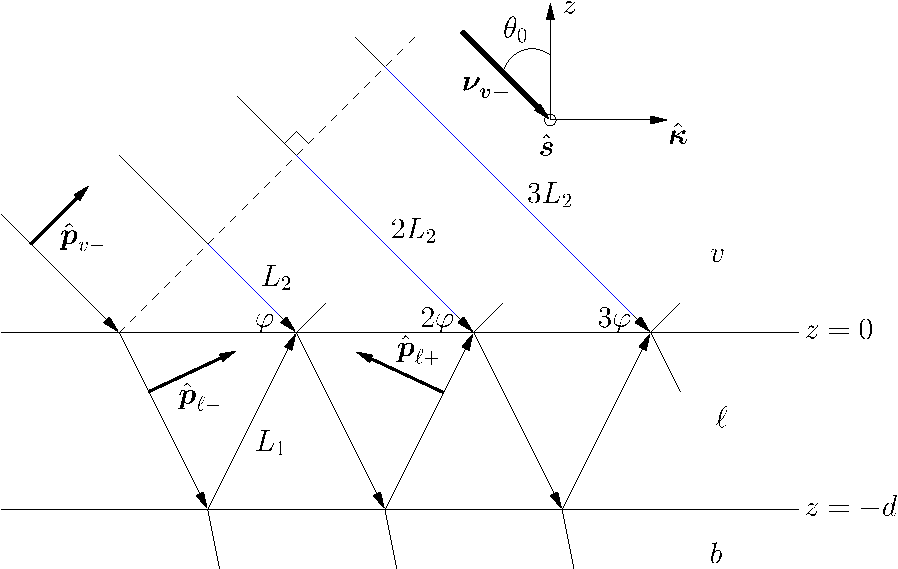
\includegraphics[width=0.65\linewidth]{../../content/figures/diag-3layer_MR_1w}
\caption[Sketch for the multiple reflected, $1\omega$ incoming field.]
{Sketch for the multiple reflected fundamental field
$\mathbf{E}_{\ell}(\omega)$, which impinges from the vacuum side along the
$\hat{\boldsymbol{\kappa}}z$-plane. $\theta_{0}$ and $\boldsymbol{\nu}_{v-}$ are
the angle of incidence and wave vector, respectively. The arrows point along the
direction of propagation. The $p$-polarization unit vectors
$\hat{\mathbf{p}}_{\beta\pm}$, point along the downward $(-)$ or upward $(+)$
directions and are denoted with thick arrows, where $\beta = v$ or $\ell$. The
$s$-polarization unit vector $\hat{\mathbf{s}}$ points out of the page.
$(1,2,3,\ldots)\varphi$ denotes the phase difference for the multiple reflected
beams with respect to the incident field, where the dotted line is perpendicular
to this beam.}
\label{fig:MR3layer1w}
\end{figure}
 

%%%%%%%%%%%%%%%%%%%%%%%%%%%%%%%%%%%%%%%%%%%%%%%%%%%%%%%%%%%%%%%%%%%%%%%%%%%%%%%%

\subsection{The SSHG Yield}

The magnitude of the radiated field is given by $E(2\omega) =
\hat{\mathbf{e}}^{\mathrm{F}}\cdot\mathbf{E}_{\ell}(2\omega)$, where
$\hat{\mathbf{e}}^{\mathrm{F}}$ is the unit vector of the final, $S$ or $P$ SH
polarization with $\mathrm{F}=S,P$, where $\hat{\mathbf{e}}^S=\hat{\mathbf{s}}$
and $\hat{\mathbf{e}}^P=\hat{\mathbf{P}}_{v+}$. We expand the rightmost term in
parenthesis of Eq. \eqref{eq:mr9} as
\begin{equation}
\begin{split}
\hat{\mathbf{P}}_{\ell +} + R^{M}_{p}\hat{\mathbf{P}}_{\ell -}
&= \frac{\sin\theta_{0}\hat{\mathbf{z}} - W_{\ell}\hat{\boldsymbol{\kappa}}}
        {N_{\ell}}
 + R^{M}_{p}
   \frac{\sin\theta_{0}\hat{\mathbf{z}} + W_{\ell}\hat{\boldsymbol{\kappa}}}
        {N_{\ell}}\\
&= \frac{1}{N_{\ell}}
\left(
\sin\theta_{0}R^{M+}_{p}\hat{\mathbf{z}}
- W_{\ell}R^{M-}_{p}\hat{\boldsymbol{\kappa}}
\right),
\end{split}
\end{equation}
where
\begin{equation}\label{eq:rm}
R^{M\pm}_{\mathrm{i}}\equiv 1 \pm R^{M}_{\mathrm{i}}, \quad \mathrm{i}=s,p.
\end{equation}
Using Eq. \eqref{eq:mf} we write Eq. \eqref{eq:mr8} as
\begin{equation}\label{eq:r10}
E_{\ell}(2\omega) = \frac{2\gamma i\omega}{cW_\ell}
\hat{\mathbf{e}}^{\mathrm{F}}\cdot\mathbf{H}_{\ell}\cdot
\boldsymbol{\mathcal{P}}_{\ell}(2\omega) 
= \frac{2\gamma i\omega}{cW_{v}}
\mathbf{e}^{\,2\omega,\mathrm{F}}_{\ell}\cdot
\boldsymbol{\mathcal{P}}_{\ell}(2\omega),
\end{equation}
where
\begin{equation}\label{eq:r12mm}
\mathbf{e}^{2\omega,\mathrm{F}}_{\ell} =\hat{\mathbf{e}}^{\mathrm{F}}\cdot 
\Bigg[
\hat{\mathbf{s}}T_{s}^{v\ell}R^{M+}_{s}\hat{\mathbf{s}} + 
\hat{\mathbf{P}}_{v+}
\frac{T^{v\ell}_{p}}
     {N_{\ell}}
\left(
\sin\theta_{0}R^{M+}_{p}\hat{\mathbf{z}}
- W_{\ell}R^{M-}_{p}\hat{\boldsymbol{\kappa}}
\right) 
\Bigg]. 
\end{equation}  
Replacing $\mathbf{E}_{\ell}(\omega)\to E_0\mathbf{e}^{\omega}_\ell$,
in Eq. \eqref{eq:tres}, we obtain that
\begin{equation}\label{eq:m4}
\boldsymbol{\mathcal{P}}_{\ell}(2\omega) = 
\left\{
\begin{array}{cc}  
E^{2}_{0}\,
\boldsymbol{\chi}_{\mathrm{surface}}:\mathbf{e}^{\omega,\mathrm{i}}_{\ell}
                                     \mathbf{e}^{\omega,\mathrm{i}}_{\ell}
& \text{(CGS units)}\\\\
\epsilon_{0}E^{2}_{0}\,
\boldsymbol{\chi}_{\mathrm{surface}}:\mathbf{e}^{\omega,\mathrm{i}}_{\ell}
                                     \mathbf{e}^{\omega,\mathrm{i}}_{\ell}
& \text{(MKS units)}\\
\end{array}
\right.,
\end{equation}
where $\mathbf{e}^{\omega}_{\ell}$ is given by Eq. \eqref{eq:vec1wcomplete},
and thus Eq. \eqref{eq:r10} reduces to ($W_{v}=\cos\theta_{0}$)
\begin{equation}\label{eq:mr10}
E_{\ell}(2\omega) 
= \frac{2\eta i \omega}{c\cos\theta_{0}}
\mathbf{e}^{2\omega,\mathrm{F}}_{\ell}\cdot
\boldsymbol{\chi}_{\mathrm{surface}}:\mathbf{e}^{\omega,\mathrm{i}}_{\ell}
                                     \mathbf{e}^{\omega,\mathrm{i}}_{\ell},
\end{equation}
where $\eta=2\pi$ in CGS units and $\eta=1/2$ in MKS units. For ease of
notation, we define
\begin{equation}\label{eq:mc0}
\Upsilon_{\mathrm{iF}}
\equiv 
\mathbf{e}^{2\omega,\mathrm{F}}_{\ell}\cdot
\boldsymbol{\chi}_{\mathrm{surface}}:\mathbf{e}^{\omega,\mathrm{i}}_{\ell}
                                     \mathbf{e}^{\omega,\mathrm{i}}_{\ell},
\end{equation}
where i stands for the incoming polarization of the fundamental electric field
given by $\hat{\mathbf{e}}^{\mathrm{i}}$ in Eq. \eqref{eq:vec1wcomplete}, and F
for the outgoing polarization of the SH electric field given by
$\hat{\mathbf{e}}^{\mathrm{F}}$ in Eq. \eqref{eq:r12mm}. I purposely omitted the
full $\boldsymbol{\chi}(-2\omega;\omega,\omega)$ notation, and will do so from
this point on.

From Eqs. \eqref{eq:rintensities} and \eqref{eq:intensity} we obtain that in
CGS units ($\eta=2\pi$), 
\begin{equation}\label{eq:r01}
\begin{split}
\vert E(2\omega)\vert^{2} &=
\vert E_{0}\vert^{4}\frac{16\pi^{2}\omega^{2}}{c^{2}W^2_{v}}
\vert\Upsilon_{\mathrm{iF}}\vert^{2}\\
%%%%%%%%%%%%%%%%%%%%%%%%%%%%%%%%%%%%%%%%%%%%%%%%%%%%%
\frac{c}{2\pi}\vert\sqrt{N_{v}}E(2\omega)\vert^{2} &=
\frac{32\pi^{3}\omega^{2}}{c^{3}\cos^2\theta_{0}}
\left\vert\frac{\sqrt{N_{v}}}{n^{2}_{\ell}}\Upsilon_{\mathrm{iF}}\right\vert^{2} 
\left(\frac{c}{2\pi}\vert\sqrt{n_{\ell}}E_{0}\vert^{2}\right)^{2}\\ 
%%%%%%%%%%%%%%%%%%%%%%%%%%%%%%%%%%%%%%%%%%%%%%%%%%%%%
I(2\omega) &=
\frac{32\pi^{3}\omega^{2}}{c^{3}\cos^2\theta_{0}}
\left\vert\frac{\sqrt{N_{v}}}{n^{2}_{\ell}}\Upsilon_{\mathrm{iF}}\right\vert^{2}
I^{2}(\omega)\\
%%%%%%%%%%%%%%%%%%%%%%%%%%%%%%%%%%%%%%%%%%%%%%%%%%%%%
\mathcal{R}_{\mathrm{iF}}(2\omega) &=
\frac{32\pi^{3}\omega^{2}}{c^{3}\cos^2\theta_{0}}
\left\vert\frac{1}{n_{\ell}}\Upsilon_{\mathrm{iF}}\right\vert^{2},
\end{split} 
\end{equation} 
and in MKS units ($\eta=1/2$),
\begin{equation}\label{r01m}
\begin{split}
\vert E(2\omega)\vert^{2} &=
\vert E_{0}\vert^{4}\frac{\omega^{2}}{c^{2}W^{2}_{v}}\\
%%%%%%%%%%%%%%%%%%%%%%%%%%%%%%%%%%%%%%%%%%%%%%%%%%%%%
2\epsilon_{0}c|\sqrt{N_{v}}E(2\omega)|^{2} &=
\frac{2\epsilon_{0}\omega^{2}}{c\cos^{2}\theta_{0}}
\left\vert\frac{\sqrt{N_{v}}}{n^{2}_{\ell}}\Upsilon_{\mathrm{iF}}\right\vert^{2} 
\frac{1}{4\epsilon^{2}_0c^{2}}
\left(2\epsilon_{0}c\vert\sqrt{n_{\ell}}E_{0}\vert^{2}\right)^{2}\\
%%%%%%%%%%%%%%%%%%%%%%%%%%%%%%%%%%%%%%%%%%%%%%%%%%%%%
I(2\omega) &= 
\frac{\omega^{2}}{2\epsilon_{0}c^3\cos^{2}\theta_{0}}
\left\vert\frac{\sqrt{N_{v}}}{n^{2}_{\ell}}\Upsilon_{\mathrm{iF}}\right\vert^{2}
I^{2}(\omega)\\
%%%%%%%%%%%%%%%%%%%%%%%%%%%%%%%%%%%%%%%%%%%%%%%%%%%%%
\mathcal{R}_{\mathrm{iF}}(2\omega) &=
\frac{\omega^{2}}{2\epsilon_{0}c^3\cos^{2}\theta_{0}}
\left\vert  \frac{1}{n_{\ell}}\Upsilon_{\mathrm{iF}}\right\vert^{2}.
\end{split}
\end{equation}
Finally, we condense these results and establish the SSHG yield as
\begin{equation}\label{eq:mc6}
\mathcal{R}_{\mathrm{iF}}(2\omega) 
\left\{
\begin{array}{ r c } 
\frac{32\pi^{3}\omega^{2}}{c^{3}\cos^{2}\theta_{0}}
\left\vert\frac{1}{n_{\ell}}\Upsilon_{\mathrm{iF}}\right\vert^{2} 
& \text{(CGS units)} \\\\
\frac{\omega^{2}}{2\epsilon_{0}c^3\cos^{2}\theta_{0}}
\left\vert\frac{1}{n_{\ell}}\Upsilon_{\mathrm{iF}}\right\vert^{2} 
& \text{(MKS units)} 
\end{array}
\right.,
\end{equation}
where $N_{v}=1$ and $W_{v}=\cos\theta_{0}$.
$\boldsymbol{\chi}_{\mathrm{surface}}$ is given in m$^{2}$/V in the MKS unit
system, since it is a surface second order nonlinear susceptibility, and
$\mathcal{R}_{\mathrm{iF}}$ is given in m$^2$/W.


%%%%%%%%%%%%%%%%%%%%%%%%%%%%%%%%%%%%%%%%%%%%%%%%%%%%%%%%%%%%%%%%%%%%%%%%%%%%%%%%
%%%%%%%%%%%%%%%%%%%%%%%%%%%%%%%%%%%%%%%%%%%%%%%%%%%%%%%%%%%%%%%%%%%%%%%%%%%%%%%%

\section{Generalized Polarization Considerations}

Ultimately, the crux of the matter is how to calculate Eq. \eqref{eq:mc0}.
Fortunately, this term can be expressed in a highly elegant and flexible manner
that greatly simplifies the required algebra. We will evaluate each potential
case and derive the necessary expressions.


%%%%%%%%%%%%%%%%%%%%%%%%%%%%%%%%%%%%%%%%%%%%%%%%%%%%%%%%%%%%%%%%%%%%%%%%%%%%%%%%

\subsection{\texorpdfstring{$2\omega$}{2w} Terms for \emph{P} and \emph{S}
Linear Polarization}

By substituting Eqs. \eqref{eq:mc1} and \eqref{eq:mmc2} into Eq.
\eqref{eq:r12mm}, we obtain
\begin{equation}\label{eq:e2wpmr}
\mathbf{e}^{2\omega,P}_{\ell} =
\frac{T^{v\ell}_{p}}{N_{\ell}}
\big(
  \sin\theta_{0}R^{M+}_{p}\hat{\mathbf{z}}
- W_{\ell}R^{M-}_{p}\cos\phi\hat{\mathbf{x}}
- W_{\ell}R^{M-}_{p}\sin\phi\hat{\mathbf{y}}
\big),
\end{equation}
for $P$ $(\hat{\mathbf{e}}^{\mathrm{F}} = \hat{\mathbf{P}}_{v+})$ outgoing
polarization, and
\begin{equation}\label{eq:e2wsmr}
\mathbf{e}^{2\omega,S}_{\ell} =
T_{s}^{v\ell}R^{M+}_{s}
\left(
- \sin\phi\hat{\mathbf{x}}
+ \cos\phi\hat{\mathbf{y}}
\right).
\end{equation}
for $S$ $(\hat{\mathbf{e}}^{\mathrm{F}}=\hat{\mathbf{s}})$ outgoing
polarization.


%%%%%%%%%%%%%%%%%%%%%%%%%%%%%%%%%%%%%%%%%%%%%%%%%%%%%%%%%%%%%%%%%%%%%%%%%%%%%%%%

\subsection{\texorpdfstring{$1\omega$}{1w} Terms for for Elliptical
Polarization}

Up until this juncture, we have not assumed any given polarization for the
incoming fields, other than that they must be in some combination of $p$ or $s$
polarization. But let us consider the most general polarization case, elliptical
polarization, by establishing that
\begin{equation}\label{eq:generalpol}
\hat{\mathbf{e}}^{\mathrm{i}}
= {\color{red}\sin\gamma}\,\hat{\mathbf{s}}
+ {\color{red}e^{i\tau}\cos\gamma}\,\hat{\mathbf{p}}_{v-}.
\end{equation}
Plugging this into Eq. \eqref{eq:vec1wcomplete} yields
\begin{equation}
\mathbf{e}^{\omega}_{\ell}
=
\Bigg[
{\color{red}\sin\gamma}\,
t^{v\ell}_{s} r^{M+}_{s}
\left(- \sin\phi\hat{\mathbf{x}} + \cos\phi\hat{\mathbf{y}}\right)
+
{\color{red}e^{i\tau}\cos\gamma}\,
\frac{t^{v\ell}_{p}}{n_{\ell}}
\left( 
  r^{M+}_{p}\sin\theta_{0}\hat{\mathbf{z}}
+ r^{M-}_{p}w_{\ell}\cos\phi\hat{\mathbf{x}}
+ r^{M-}_{p}w_{\ell}\sin\phi\hat{\mathbf{y}}
\right)
\Bigg].
\end{equation}
Eq. \eqref{eq:mc0} makes it clear that what we really need is
$\mathbf{e}^{\omega}_{\ell}\mathbf{e}^{\omega}_{\ell}$. Multiplying these terms
out leads to the following expression,
\begin{equation}
\begin{split}
\mathbf{e}^{\omega}_{\ell}
\mathbf{e}^{\omega}_{\ell}
&=
{\color{red}\sin^{2}\gamma}\,
\left(t^{v\ell}_{s}r^{M+}_{s}\right)^{2}
\big(
  \sin^{2}\phi\hat{\mathbf{x}}\hat{\mathbf{x}}
 + \cos^{2}\phi\hat{\mathbf{y}}\hat{\mathbf{y}}
 - 2\sin\phi\cos\phi\hat{\mathbf{x}}\hat{\mathbf{y}}
\big)\\
&+
{\color{red}e^{2i\tau} \cos^{2}\gamma}\,
\left(\frac{t^{v\ell}_{p}}{n_{\ell}}\right)^{2}
\bigg(
\big(r^{M-}_{p}\big)^{2}w^{2}_{\ell}\cos^{2}\phi
    \hat{\mathbf{x}}\hat{\mathbf{x}}
  + \big(r^{M-}_{p}\big)^{2}w^{2}_{\ell}\sin^{2}\phi
    \hat{\mathbf{y}}\hat{\mathbf{y}}
  + \big(r^{M+}_{p}\big)^{2}\sin^{2}\theta_{0}
    \hat{\mathbf{z}}\hat{\mathbf{z}}\\
  &\hspace{3.5cm}+ 2r^{M+}_{p}r^{M-}_{p}w_{\ell}\sin\theta_{0}\sin\phi
    \hat{\mathbf{y}}\hat{\mathbf{z}}
  + 2r^{M+}_{p}r^{M-}_{p}w_{\ell}\sin\theta_{0}\cos\phi
    \hat{\mathbf{x}}\hat{\mathbf{z}}
  + 2\big(r^{M-}_{p}\big)^{2}w^{2}_{\ell}\sin\phi\cos\phi
    \hat{\mathbf{x}}\hat{\mathbf{y}}
\bigg)\\
&+
{\color{red}2e^{i\tau}\sin\gamma\cos\gamma}\,
\frac{t^{v\ell}_{p}t^{v\ell}_{s}r^{M+}_{s}}{n_{\ell}}
\Big(
  - r^{M-}_{p}w_{\ell}\sin\phi\cos\phi
    \hat{\mathbf{x}}\hat{\mathbf{x}}
  + r^{M-}_{p}w_{\ell}\sin\phi\cos\phi
    \hat{\mathbf{y}}\hat{\mathbf{y}}\\
  &\hspace{4.5cm}+ r^{M+}_{p}\sin\theta_{0}\cos\phi
    \hat{\mathbf{y}}\hat{\mathbf{z}}
  - r^{M+}_{p}\sin\theta_{0}\sin\phi
    \hat{\mathbf{x}}\hat{\mathbf{z}}
  + r^{M-}_{p}w_{\ell}\cos 2\phi
    \hat{\mathbf{x}}\hat{\mathbf{y}}
\Big).
\end{split}
\end{equation}
It is very convenient to switch over to a matrix representation. We can readily
express the previous equation as a combination of vectors,
\begin{equation}
\mathbf{e}^{\omega}_{\ell}
\mathbf{e}^{\omega}_{\ell}
=
\mathbf{C}\mathbf{R},
\end{equation}
where
\begin{equation}
\mathbf{C} = 
\big(
\hat{\mathbf{x}}\hat{\mathbf{x}}\hspace{5pt}
\hat{\mathbf{y}}\hat{\mathbf{y}}\hspace{5pt}
\hat{\mathbf{z}}\hat{\mathbf{z}}\hspace{5pt}
\hat{\mathbf{y}}\hat{\mathbf{z}}\hspace{5pt}
\hat{\mathbf{x}}\hat{\mathbf{z}}\hspace{5pt}
\hat{\mathbf{x}}\hat{\mathbf{y}}
\big),
\end{equation}
and
\begin{equation}\label{eq:Rcomplete}
\begin{split}
\mathbf{R}
&=
{\color{red}\sin^{2}\gamma}\,
\left(t^{v\ell}_{s}r^{M+}_{s}\right)^{2}
\begin{pmatrix}
\sin^{2}\phi        \\[8pt]
\cos^{2}\phi        \\[8pt]
0                   \\[8pt]
0                   \\[8pt]
0                   \\[8pt]
- 2\sin\phi\cos\phi 
\end{pmatrix}\\[8pt]
&+
{\color{red}e^{2i\tau}\cos^{2}\gamma}\,
\left(\frac{t^{v\ell}_{p}}{n_{\ell}}\right)^{2}
\begin{pmatrix}
\left(r^{M-}_{p}\right)^{2}w^{2}_{\ell}\cos^{2}\phi       \\[8pt]    
\left(r^{M-}_{p}\right)^{2}w^{2}_{\ell}\sin^{2}\phi       \\[8pt]
\left(r^{M+}_{p}\right)^{2}\sin^{2}\theta_{0}             \\[8pt]
2r^{M+}_{p}r^{M-}_{p}w_{\ell}\sin\theta_{0}\sin\phi       \\[8pt]
2r^{M+}_{p}r^{M-}_{p}w_{\ell}\sin\theta_{0}\cos\phi       \\[8pt]
2\left(r^{M-}_{p}\right)^{2}w^{2}_{\ell}\sin\phi\cos\phi  
\end{pmatrix}\\[8pt]
&+
{\color{red}2e^{i\tau}\sin\gamma\cos\gamma}\,
\frac{t^{v\ell}_{p}t^{v\ell}_{s}r^{M+}_{s}}{n_{\ell}}
\begin{pmatrix}
-r^{M-}_{p}w_{\ell}\sin\phi\cos\phi \\[8pt]
r^{M-}_{p}w_{\ell}\sin\phi\cos\phi  \\[8pt]
0                                   \\[8pt]
r^{M+}_{p}\sin\theta_{0}\cos\phi    \\[8pt]
-r^{M+}_{p}\sin\theta_{0}\sin\phi   \\[8pt]
r^{M-}_{p}w_{\ell}\cos 2\phi        
\end{pmatrix}.
\end{split}
\end{equation}
Now that Eq. \eqref{eq:Rcomplete} can encompass all possible polarization
choices, we can obtain some common polarization cases using some specific values
for $\gamma$ and $\tau$ featured in Table \ref{tab:polcases}.

\begin{table}
\caption{Values for $\gamma$ and $\tau$ (see Eq. \eqref{eq:generalpol}) that
yield common polarization cases.\label{tab:polcases}}
\begin{tabular}{ | l l | c c | }
\hline
\multicolumn{2}{|c|}{Type}                    & $\gamma$  & $\tau$    \\
\hline
Linear        & $p$ ($\hat{\mathbf{p}}_{v-}$) & 0         & 0         \\
Linear        & $s$ ($\hat{\mathbf{s}}$)      & $\pi/2$   & 0         \\
Linear        & $p$ + $s$ & $\pi/4$           & 0         \\
\hline
Circular      & Left                          & $\pi/4$   & $-\pi/2$  \\
Circular      & Right                         & $\pi/4$   & $+\pi/2$  \\
\hline
Elliptical    &                               & Any       & Any       \\
\hline
\end{tabular}
\end{table}


%%%%%%%%%%%%%%%%%%%%%%%%%%%%%%%%%%%%%%%%%%%%%%%%%%%%%%%%%%%%%%%%%%%%%%%%%%%%%%%%

\subsection{\texorpdfstring{$1\omega$}{1w} Terms for for \emph{p} and \emph{s}
Linear Polarization}

Given that the terms for $1\omega$ are now presented for the most general
polarization case, we can easily recover the expressions for $p$ and $s$ linear
polarization by plugging in the appropriate values for $\gamma$ and $\tau$
(featured in Table \ref{tab:polcases}) into Eq. \eqref{eq:Rcomplete}. With
$\gamma = 0$ and $\tau = 0$ we obtain
\begin{equation}\label{eq:ewewpmr}
\begin{split}
\mathbf{e}^{\omega,\mathrm{p}}_{\ell}\mathbf{e}^{\omega,\mathrm{p}}_{\ell} =
\left(\frac{t^{v\ell}_{p}}{n_{\ell}}\right)^{2}
\bigg(
  \big(&r^{M-}_{p}\big)^{2}w^{2}_{\ell}\cos^{2}\phi
  \hat{\mathbf{x}}\hat{\mathbf{x}}
+ 2\big(r^{M-}_{p}\big)^{2}w^{2}_{\ell}\sin\phi\cos\phi
  \hat{\mathbf{x}}\hat{\mathbf{y}}\\
+ 2&r^{M+}_{p}r^{M-}_{p}w_{\ell}\sin\theta_{0}\cos\phi
  \hat{\mathbf{x}}\hat{\mathbf{z}}
+ \big(r^{M-}_{p}\big)^{2}w^{2}_{\ell}\sin^{2}\phi
  \hat{\mathbf{y}}\hat{\mathbf{y}}\\
+ 2&r^{M+}_{p}r^{M-}_{p}w_{\ell}\sin\theta_{0}\sin\phi
  \hat{\mathbf{y}}\hat{\mathbf{z}}
+ \big(r^{M+}_{p}\big)^{2}\sin^{2}\theta_{0}
   \hat{\mathbf{z}}\hat{\mathbf{z}}
\bigg),
\end{split}
\end{equation}
for $p$ incoming polarization (equivalent to using
$\hat{\mathbf{e}}^{\mathrm{i}} = \hat{\mathbf{p}}_{v-}$ in Eq.
\eqref{eq:vec1wcomplete}), and with $\gamma = \pi/2$ and $\tau = 0$ we obtain
\begin{equation}\label{eq:ewewsmr}
\mathbf{e}^{\omega,\mathrm{s}}_{\ell}\mathbf{e}^{\omega,\mathrm{s}}_{\ell}
= \left(t^{v\ell}_{s}r^{M+}_{s}\right)^{2}
\big(
  \sin^{2}\phi\hat{\mathbf{x}}\hat{\mathbf{x}}
 + \cos^{2}\phi\hat{\mathbf{y}}\hat{\mathbf{y}}
 - 2\sin\phi\cos\phi\hat{\mathbf{x}}\hat{\mathbf{y}}
\big).
\end{equation}
for $s$ incoming polarization (equivalent to using
$\hat{\mathbf{e}}^{\mathrm{i}} = \hat{\mathbf{s}}$ in Eq.
\eqref{eq:vec1wcomplete}).


%%%%%%%%%%%%%%%%%%%%%%%%%%%%%%%%%%%%%%%%%%%%%%%%%%%%%%%%%%%%%%%%%%%%%%%%%%%%%%%%
%%%%%%%%%%%%%%%%%%%%%%%%%%%%%%%%%%%%%%%%%%%%%%%%%%%%%%%%%%%%%%%%%%%%%%%%%%%%%%%%

\section{\texorpdfstring{$\mathcal{R}_{\mathrm{iF}}$}{R} for Different
Polarization Cases}\label{sec:rcases}

We now have everything we need to derive explicit expressions for
$\mathcal{R}_{\mathrm{iF}}$, Eq. \eqref{eq:mc6}, for the any polarization combination of incoming and outgoing fields. Particularly, the four different combinations of linear polarization (iF=$pP$, $pS$, $sP$, and $sS$) can be easily recovered from this treatment.
For this, we must expand $\Upsilon_{\mathrm{iF}}$ from Eq. \eqref{eq:mc0} for
each case.

We summarize the combination of equations needed to derive the expressions for
all four polarization cases of $\mathcal{R}_{\mathrm{iF}}$ in Table
\ref{tab:summary}. In the following subsections we will derive the explicit
expressions for $\Upsilon_{\mathrm{iF}}$ for the most general case where the
surface has no symmetry. We will then develop these expressions for particular
cases of the most commonly investigated surfaces, the (111), (001) and (110)
crystallographic faces. For ease of notation, we split $\Upsilon_{\mathrm{iF}}$
as
\begin{equation}\label{eq:mc25}
\Upsilon_{\mathrm{iF}} = \Gamma_{\mathrm{iF}}\,r_{\mathrm{iF}},
\end{equation}
and omit the ``surface''subscript for the $\chi^{\mathrm{abc}}$ components. The
avid reader should refer to Ref. \cite{andersonthesis} if interested in
reviewing the step-by-step derivation of the expressions listed below.

\begin{table}[b]
\caption{(Color online) Polarization unit vectors for
$\hat{\mathbf{e}}^{\mathrm{F}}$ and $\hat{\mathbf{e}}^{\mathrm{i}}$, and
equations describing $\mathbf{e}^{2\omega,\mathrm{F}}_{\ell}$ and
$\mathbf{e}^{\omega,\mathrm{i}}_{\ell}\mathbf{e}^{\omega,\mathrm{i}}_{\ell}$ for
each polarization case.}
\label{tab:summary}
\centering
\begin{tabular}{| c | l | l | c | c |}
\hline
Case               & $\hat{\mathbf{e}}^{\mathrm{F}}$
                   & $\hat{\mathbf{e}}^{\mathrm{i}}$
                   & $\mathbf{e}^{2\omega,\mathrm{F}}_{\ell}$
                   & $\mathbf{e}^{\omega,\mathrm{i}}_{\ell}
                      \mathbf{e}^{\omega,\mathrm{i}}_{\ell}$ \\
\hline
$\mathcal{R}_{pP}$ & $\hat{\mathbf{P}}_{v+}$
                   & $\hat{\mathbf{p}}_{v-}$
                   &  Eq. \eqref{eq:e2wpmr} & Eq. \eqref{eq:ewewpmr} \\
$\mathcal{R}_{pS}$ & $\hat{\mathbf{S}}$
                   & $\hat{\mathbf{p}}_{v-}$
                   &  Eq. \eqref{eq:e2wsmr} & Eq. \eqref{eq:ewewpmr} \\
$\mathcal{R}_{sP}$ & $\hat{\mathbf{P}}_{v+}$
                   & $\hat{\mathbf{s}}$
                   &  Eq. \eqref{eq:e2wpmr} & Eq. \eqref{eq:ewewsmr} \\
$\mathcal{R}_{sS}$ & $\hat{\mathbf{S}}$
                   & $\hat{\mathbf{s}}$
                   &  Eq. \eqref{eq:e2wsmr} & Eq. \eqref{eq:ewewsmr} \\
\hline
\end{tabular}
\end{table}

Many expressions can be greatly simplified by introducing a matrix
representation for $\boldsymbol{\chi}$. Disregarding all symmetry relations, we
have
\begin{equation}
\boldsymbol{\chi} =
\begin{pmatrix}
\chi^{xxx}&\chi^{xyy}&\chi^{xzz} &|& \chi^{xyz}&\chi^{xxz}&\chi^{xxy} \\[3pt]
\chi^{yxx}&\chi^{yyy}&\chi^{yzz} &|& \chi^{yyz}&\chi^{yxz}&\chi^{yxy} \\[3pt]
\chi^{zxx}&\chi^{zyy}&\chi^{zzz} &|& \chi^{zyz}&\chi^{zxz}&\chi^{zxy}
\end{pmatrix}
,
\end{equation}
where all 18 independent components are accounted for, recalling that
$\chi^{\mathrm{abc}} = \chi^{\mathrm{acb}}$ for SHG. Notice that the left hand
block contains the components of $\chi^{\mathrm{abc}}$ where $b = c$, and the
right hand block those where $b \neq c$. As mentioned above, we are interested
in the (111), (110) and (001) crystallographic faces, that belong to the
$C_{3v}$, $C_{2v}$, and $C_{4v}$ symmetry groups, respectively. For the (111)
surface, we choose the $x$ and $y$ axes along the [$11\bar{2}$] and
[$1\bar{1}0$] directions, respectively. For the (110) and (001), we consider the
$y$ axis perpendicular to the plane of symmetry.\cite{sipePRB87} These are
represented in matrix form as
\begin{equation}\label{eq:111matrix}
\boldsymbol{\chi}^{(111)} =
\begin{pmatrix}
\chi^{xxx}&-\chi^{xxx}&    0      &|&     0     &\chi^{xxz}&     0     \\[3pt]
     0    &      0    &    0      &|& \chi^{xxz}&     0   &-\chi^{xxx}\\[3pt]
\chi^{zxx}& \chi^{zxx}&\chi^{zzz} &|&     0     &     0    &     0 
\end{pmatrix}
,
\end{equation}
\begin{equation}\label{eq:110matrix}
\boldsymbol{\chi}^{(110)} =
\begin{pmatrix}
     0    &     0    &     0     &|&      0    &\chi^{xxz}&     0     \\[3pt]
     0    &     0    &     0     &|& \chi^{yyz}&     0    &     0     \\[3pt]
\chi^{zxx}&\chi^{zyy}&\chi^{zzz} &|&      0    &     0    &     0
\end{pmatrix}
,
\end{equation}
and
\begin{equation}\label{eq:001matrix}
\boldsymbol{\chi}^{(001)} =
\begin{pmatrix}
     0    &     0    &     0     &|&      0    &\chi^{xxz}&     0     \\[3pt]
     0    &     0    &     0     &|& \chi^{xxz}&     0    &     0     \\[3pt]
\chi^{zxx}&\chi^{zxx}&\chi^{zzz} &|&      0    &     0    &     0
\end{pmatrix}
.
\end{equation}
In general, $\boldsymbol{\chi}^{(111)}\ne \boldsymbol{\chi}^{(110)} \ne 
\boldsymbol{\chi}^{(001)}$.


%%%%%%%%%%%%%%%%%%%%%%%%%%%%%%%%%%%%%%%%%%%%%%%%%%%%%%%%%%%%%%%%%%%%%%%%%%%%%%%%

\subsection{\texorpdfstring{$\mathcal{R}_{pP}$ ($p$-in, $P$-out)}
{RpP (p-in, P-out)}}
\label{sec:RpP} 

Per Table \ref{tab:summary}, $\mathcal{R}_{pP}$ requires Eqs. \eqref{eq:e2wpmr}
and \eqref{eq:ewewpmr}. After some algebra, we obtain that
\begin{equation}\label{eq:mc78}
\Gamma_{pP} =
\frac{T^{v\ell}_{p}}{N_{\ell}}
\left(\frac{t^{v\ell}_{p}}{n_{\ell}}\right)^{2}
,
\end{equation}
and
\begin{widetext}
\begin{equation}\label{eq:rppmatrix}
r_{pP} =
\begin{pmatrix}
-R^{M-}_{p}W_{\ell}\cos\phi \\[3pt]
-R^{M-}_{p}W_{\ell}\sin\phi \\[3pt]
+R^{M+}_{p}\sin\theta_{0}
\end{pmatrix}
\circ
\boldsymbol{\chi}
\cdot
\begin{pmatrix}
\left(r^{M-}_{p}\right)^{2}w^{2}_{\ell}\cos^{2}\phi\\[8pt]
\left(r^{M-}_{p}\right)^{2}w^{2}_{\ell}\sin^{2}\phi\\[8pt]
\left(r^{M+}_{p}\right)^{2}\sin^{2}\theta_{0}\\[8pt]
2r^{M+}_{p}r^{M-}_{p}w_{\ell}\sin\theta_{0}\sin\phi\\[8pt]
2r^{M+}_{p}r^{M-}_{p}w_{\ell}\sin\theta_{0}\cos\phi\\[8pt]
2\left(r^{M-}_{p}\right)^{2}w^{2}_{\ell}\sin\phi\cos\phi
\end{pmatrix}
,
\end{equation}
\end{widetext}
where all 18 independent components of $\boldsymbol{\chi}$ can contribute to
$\mathcal{R}_{pP}$. The ``$\circ$'' symbol is the Hadamard (piecewise) matrix
product. For the (111) surface, we substitute Eq. \eqref{eq:111matrix} in Eq.
\eqref{eq:rppmatrix} in lieu of $\boldsymbol{\chi}$ to obtain
\begin{widetext}
\begin{equation}\label{eq:rpp111}
\begin{split}
r^{(111)}_{pP} &= 
R^{M+}_{p}\sin\theta_{0}
\Big[
  \left(r^{M+}_{p}\right)^{2}\sin^{2}\theta_{0}\chi^{zzz}
+ \left(r^{M-}_{p}\right)^{2}w^{2}_{\ell}\chi^{zxx}
\Big]\\
&- R^{M-}_{p}w_{\ell}W_{\ell}
\Big[
  2r^{M+}_{p}r^{M-}_{p}\sin\theta_{0}\chi^{xxz}
+ \left(r^{M-}_{p}\right)^{2}w_{\ell}\chi^{xxx}\cos3\phi
\Big],
\end{split}
\end{equation}
\end{widetext}
where the three-fold azimuthal symmetry of the SHG signal that is typical of the
$C_{3v}$ symmetry group is seen in the $3\phi$ argument of the cosine function.
For the (110) surface, we substitute Eq. \eqref{eq:110matrix} in Eq. 
\eqref{eq:rppmatrix} to obtain
\begin{widetext}
\begin{equation}\label{eq:rpp110}
\begin{split}
r^{(110)}_{pP} &= 
R^{M+}_{p}\sin\theta_{0}
\Bigg[
  \left(r^{M+}_{p}\right)^{2}\sin^{2}\theta_{0}\chi^{zzz}
+ \left(r^{M-}_{p}\right)^{2}w^{2}_{\ell}
\left(
\frac{\chi^{zyy} + \chi^{zxx}}{2} + \frac{\chi^{zyy} - \chi^{zxx}}{2}\cos2\phi 
\right) 
\Bigg]\\
&- 2R^{M-}_{p}r^{M+}_{p}r^{M-}_{p}w_{\ell}W_{\ell}\sin\theta_{0}
\left(
\frac{\chi^{yyz} + \chi^{xxz}}{2} + \frac{\chi^{yyz} - \chi^{xxz}}{2}\cos2\phi 
\right). 
\end{split}
\end{equation}
\end{widetext}
The two-fold azimuthal symmetry of the SHG signal that is typical of the
$C_{2v}$ symmetry group, is seen in the $2\phi$ argument of the cosine function.
Lastly, for the (001) surface we simply make $\chi^{zxx} = \chi^{zyy}$ and
$\chi^{xxz} = \chi^{yyz}$ (see Eqs. \eqref{eq:110matrix} and
\eqref{eq:001matrix}), and the previous expression reduces to
\begin{widetext}
\begin{equation}\label{rpp001}
r^{(001)}_{pP} = 
R^{M+}_{p}\sin\theta_{0}
\bigg[
  \left(r^{M+}_{p}\right)^{2}\sin^{2}\theta_{0}\chi^{zzz}
+ \left(r^{M-}_{p}\right)^{2}w^{2}_{\ell}\chi^{zxx}
\bigg]
- 2R^{M-}_{p}r^{M+}_{p}r^{M-}_{p}w_{\ell}W_{\ell}\sin\theta_{0}\chi^{xxz}.
\end{equation}
\end{widetext}
This time, the azimuthal $4\phi$ symmetry for the $C_{4v}$ group of the (001)
surface is absent in this  expression since this contribution is only related to
the bulk nonlinear quadrupolar SH term,\cite{sipePRB87} which we neglect in this
work.


%%%%%%%%%%%%%%%%%%%%%%%%%%%%%%%%%%%%%%%%%%%%%%%%%%%%%%%%%%%%%%%%%%%%%%%%%%%%%%%%

\subsection{\texorpdfstring{$\mathcal{R}_{sP}$ ($s$-in, $P$-out)} {RsP (s-in,
P-out)}}
\label{sec:RsP}

Per Table \ref{tab:summary}, $\mathcal{R}_{sP}$ requires Eqs. \eqref{eq:e2wpmr}
and \eqref{eq:ewewsmr}. After some algebra, we obtain that
\begin{equation}\label{mcv4}
\Gamma_{sP}=
\frac{T^{v\ell}_{p}}{N_{\ell}}
\left(t^{v\ell}_{s}r^{M+}_{s}\right)^{2},
\end{equation}
and
\begin{equation}\label{eq:rspmatrix}
r_{sP} =
\begin{pmatrix}
-R^{M-}_{p}W_{\ell}\cos\phi \\[3pt]
-R^{M-}_{p}W_{\ell}\sin\phi \\[3pt]
+R^{M+}_{p}\sin\theta_{0}
\end{pmatrix}
\circ
\boldsymbol{\chi}
\cdot
\begin{pmatrix}
\sin^{2}\phi\\
\cos^{2}\phi\\
0\\
0\\
0\\
- 2\sin\phi\cos\phi
\end{pmatrix}
.
\end{equation}
In this case, 9 out of the 18 components of $\boldsymbol{\chi}$ can contribute
to $\mathcal{R}_{sP}$. This is because there is no $E^z_v(\omega)$ component,
as the incoming polarization is $s$. As before, we substitute Eqs.
\eqref{eq:111matrix}, \eqref{eq:110matrix}, and \eqref{eq:001matrix} in Eq.
\eqref{eq:rspmatrix} to obtain
\begin{equation}\label{eq:rsp111}
r^{(111)}_{sP} = 
R^{M+}_{p}\sin\theta_{0}\chi^{zxx} +
R^{M-}_{p}W_{\ell}\chi^{xxx}\cos3\phi
\end{equation}
for the (111) surface,
\begin{equation}\label{eq:rsp110}
r^{(110)}_{sP} = 
R^{M+}_{p}\sin\theta_{0}
\left(
\frac{\chi^{zxx} + \chi^{zyy}}{2} + \frac{\chi^{zyy} - \chi^{zxx}}{2}\cos2\phi
\right)
\end{equation}
for the (110) surface, and
\begin{equation}\label{eq:rsp001}
r^{(001)}_{sP} = R^{M+}_{p}\sin\theta_{0}\chi^{zxx}
\end{equation}
for the (001) surface.


%%%%%%%%%%%%%%%%%%%%%%%%%%%%%%%%%%%%%%%%%%%%%%%%%%%%%%%%%%%%%%%%%%%%%%%%%%%%%%%%

\subsection{\texorpdfstring{$\mathcal{R}_{pS}$ ($p$-in, $S$-out)} {RpS (p-in,
S-out)}}
\label{sec:RpS}

Per Table \ref{tab:summary}, $\mathcal{R}_{pS}$ requires Eqs. \eqref{eq:e2wsmr}
and \eqref{eq:ewewpmr}. After some algebra, we obtain that
\begin{equation}\label{mcv}
\Gamma_{pS} =
T_{s}^{v\ell}R^{M+}_{s}
\left(\frac{t^{v\ell}_{p}}{n_{\ell}}\right)^{2},
\end{equation}
and
\begin{equation}\label{eq:rpsmatrix}
r_{pS}=
\begin{pmatrix}
-\sin\phi\\
\cos\phi\\
0
\end{pmatrix}
\circ
\boldsymbol{\chi}
\cdot
\begin{pmatrix}
\left(r^{M-}_{p}\right)^{2}w^{2}_{\ell}\cos^{2}\phi\\[8pt]
\left(r^{M-}_{p}\right)^{2}w^{2}_{\ell}\sin^{2}\phi\\[8pt]
\left(r^{M+}_{p}\right)^{2}\sin^{2}\theta_{0}\\[8pt]
2r^{M+}_{p}r^{M-}_{p}w_{\ell}\sin\theta_{0}\sin\phi\\[8pt]
2r^{M+}_{p}r^{M-}_{p}w_{\ell}\sin\theta_{0}\cos\phi\\[8pt]
2\left(r^{M-}_{p}\right)^{2}w^{2}_{\ell}\sin\phi\cos\phi
\end{pmatrix}
,
\end{equation}
In this case, 12 out of the 18 components of $\boldsymbol{\chi}$ can contribute
to $\mathcal{R}_{pS}$. This is because there is no
$\mathcal{P}^{z}_\ell(2\omega)$ component, as the outgoing polarization is $S$.
As before, we substitute Eqs. \eqref{eq:111matrix}, \eqref{eq:110matrix}, and
\eqref{eq:001matrix} in Eq. \eqref{eq:rpsmatrix} to obtain
\begin{equation}\label{eq:rps111}
r^{(111)}_{pS} = - \left(r^{M-}_{p}\right)^{2}w^{2}_{\ell}\chi^{xxx}\sin3\phi
\end{equation}
for the (111) surface,
\begin{equation}\label{eq:rps110}
r^{(110)}_{pS} =
r^{M+}_{p}r^{M-}_{p}w_{\ell}\sin\theta_{0}(\chi^{yyz} - \chi^{xxz})\sin2\phi
\end{equation}
for the (110) surface, and finally,
\begin{equation}\label{eq:rps001}
r^{(001)}_{pS} = 0
\end{equation}
for the (001) surface, where the zero value is only surface related, as we
neglect the bulk nonlinear quadrupolar contribution.\cite{sipePRB87}


%%%%%%%%%%%%%%%%%%%%%%%%%%%%%%%%%%%%%%%%%%%%%%%%%%%%%%%%%%%%%%%%%%%%%%%%%%%%%%%%

\subsection{\texorpdfstring{$\mathcal{R}_{sS}$ ($s$-in, $S$-out)}{RsS (s-in,
S-out)}}
\label{sec:RsS}

Per Table \ref{tab:summary}, $\mathcal{R}_{sS}$ requires Eqs. \eqref{eq:e2wsmr}
and \eqref{eq:ewewsmr}. After some algebra, we obtain that
\begin{equation}
\Gamma_{sS} = 
T_{s}^{v\ell}R^{M+}_{s}\left(t^{v\ell}_{s}r^{M+}_{s}\right)^{2},
\end{equation}
and
\begin{equation}\label{eq:rssmatrix}
r_{sS}=
\begin{pmatrix}
-\sin\phi\\
\cos\phi\\
0
\end{pmatrix}
\circ
\boldsymbol{\chi}
\cdot
\begin{pmatrix}
\sin^{2}\phi\\
\cos^{2}\phi\\
0\\
0\\
0\\
- 2\sin\phi\cos\phi
\end{pmatrix}
.
\end{equation}
In this case, only 6 out of the 18 components of $\boldsymbol{\chi}$ can
contribute to $\mathcal{R}_{sS}$. This is because there is neither an
$E^{z}_v(\omega)$ component as the incoming polarization is $s$, nor a
$\mathcal{P}^{z}_\ell(2\omega)$ component as the outgoing polarization is $S$.
As before, we substitute Eqs. \eqref{eq:111matrix}, \eqref{eq:110matrix}, and
\eqref{eq:001matrix} in Eq. \eqref{eq:rssmatrix} to obtain
\begin{equation}\label{eq:rss111}
r^{(111)}_{sS} = \chi^{xxx}\sin3\phi
\end{equation}
for the (111) surface, and 
\begin{equation}\label{eq:rss110}
r^{(110)}_{sS} = 0
\end{equation}
and
\begin{equation}\label{eq:rss001}
r^{(001)}_{sS} = 0
\end{equation}
for the (110) and (001) surfaces, respectively, both being zero as the bulk
nonlinear quadrupolar contribution is not considered here.\cite{sipePRB87}


%%%%%%%%%%%%%%%%%%%%%%%%%%%%%%%%%%%%%%%%%%%%%%%%%%%%%%%%%%%%%%%%%%%%%%%%%%%%%%%%
%%%%%%%%%%%%%%%%%%%%%%%%%%%%%%%%%%%%%%%%%%%%%%%%%%%%%%%%%%%%%%%%%%%%%%%%%%%%%%%%

\section{Conclusions}

In this manuscript, we derived the complete expressions for the SSHG radiation
using the three layer model to describe the radiating system. Our derivation
yields the full expressions for the radiation that include all required
components of $\chi^{\mathrm{abc}}$, regardless of symmetry considerations.
Thus, these expressions can be applied to any surface symmetry. We also reduce
them according to the most commonly used surface symmetries, the (111), (110),
and (100) cases.


%%%%%%%%%%%%%%%%%%%%%%%%%%%%%%%%%%%%%%%%%%%%%%%%%%%%%%%%%%%%%%%%%%%%%%%%%%%%%%%%
%%%%%%%%%%%%%%%%%%%%%%%%%%%%%%%%%%%%%%%%%%%%%%%%%%%%%%%%%%%%%%%%%%%%%%%%%%%%%%%%


\bibliographystyle{unsrt}
\bibliography{/Users/sma/Dropbox/Docs/academics/master}

\end{document}
